% This chapter explains all the work related to what is implied in this
% research. This includes all the procedures involved in the serveral
% phases of the experiment realized in order to obtain and analyze data.
% Under this context, several publications were studied, and their study
% is resumed in the following subsections.

\section{Datasets of acted emotions}

{\color{JungleGreen} Añadir. }


\section{Image classification}

{\color{JungleGreen}
Añadir papers sobre aruquitecturas de CNNs para clasificación de imágenes:
\begin{itemize}
  \item LeNet
  \item AlexNet
  \item VGG
  \item GoogleNet
  \item Network in Network
\end{itemize}
}


\section{Facial emotion recognition}

{\color{JungleGreen}
Añadir papers sobre arquitecturas de CNNs para reconocimiento de emociones:
\begin{itemize}
  \item Going Deeper in FER w/DNNs
  \item FER w/CNNs
  \item Supervised Comitee
  \item Multi-modality network {\color{blue}(Brief)}
  \item 3D CNNs {\color{blue}(Brief)}
  \item Micro expression detection based on DL {\color{blue}(Brief)}
  \item Deep Face {\color{blue}(Brief)}
\end{itemize}
}


\section{Artificial intelligence in portable devices}

The recent developments in small mobile devices and wireless communications
provide a strong motivation to develop new software techniques and mobile
services in many areas. Pervasive computing is often mentioned in the
context of improving healthcare. In pervasive healthcare computing, a nobel
approach for diagnosing diabetes is using neural networks in portable devices
\citep{Karan2012}. This serves as an example of the importance on developing
nobel models that are available to run in portable devices, since the
application of neural networks helps solving many problems in various areas.

CNN based recognition systems need large amounts of memory and computational
power. Considering hardware constraints, people have proposed ANN model
architectures to improve deploymente and performance in portable devices
\citep{Rastegari2016, Wu2016, Kim2015}.

{\color{Orchid}
Despite several computational cost, memory footprint, and
storage reductions, improving DCNNs in this regard continues to be an open
area of research, especially with the aim of deploying them on FPGAs,
embedded systems, mobile devices, and other devices with limited memory and
battery constraints. Some of the very recent developments in this regard
include DCNN compression and weight quantization, fast algorithms, GPU
clusters with truncated representations, and FPGA accelerated advances
\citep{Waseem2017}.}


\subsubsection{XNOR-Net}

\cite{Rastegari2016} propose two approximations to standard convolutional
neural networks: Binary-Weight-Networks (NNs with binary weights) and
XNOR-Networks. \footnote{Their code is available at:
\url{http://allenai.org/plato/xnornet}.}

A convolutional neural network with binary weights is
significantly smaller ($\sim 32 \times$) than an equivalent network
with single-precision weight values. In addition, binary weight values imply
convolutions computed by only addition and subtraction, resulting in $\sim
2 \times$ speed up.

In XNOR-Networks, both the weights and the inputs to the convolutional
and fully connected layers are approximated with binary values. Binary
weights and binary inputs allow an efficient way of implementing
convolutional operations. If all of the operands of the convolutions are
binary, then the convolutions can be estimated by XNOR and bitcounting
operations \citep{Courbariaux2016}. XNOR-Nets result in accurate
approximation of CNNs while offering $\sim 58 \times$ speed up in CPUs
(in terms of number of the high precision operations).

Figure \ref{fig:binaryCNN} displays the architecture of a standard CNN and
the architecture of the two proposed models, the Binary-Weight-Networks,
and the XNOR-Network, along with their respective memory and computing
saving, and their accuracy over the ImageNet dataset with a modified AlexNet.

\begin{figure}[!h]
	\centering
	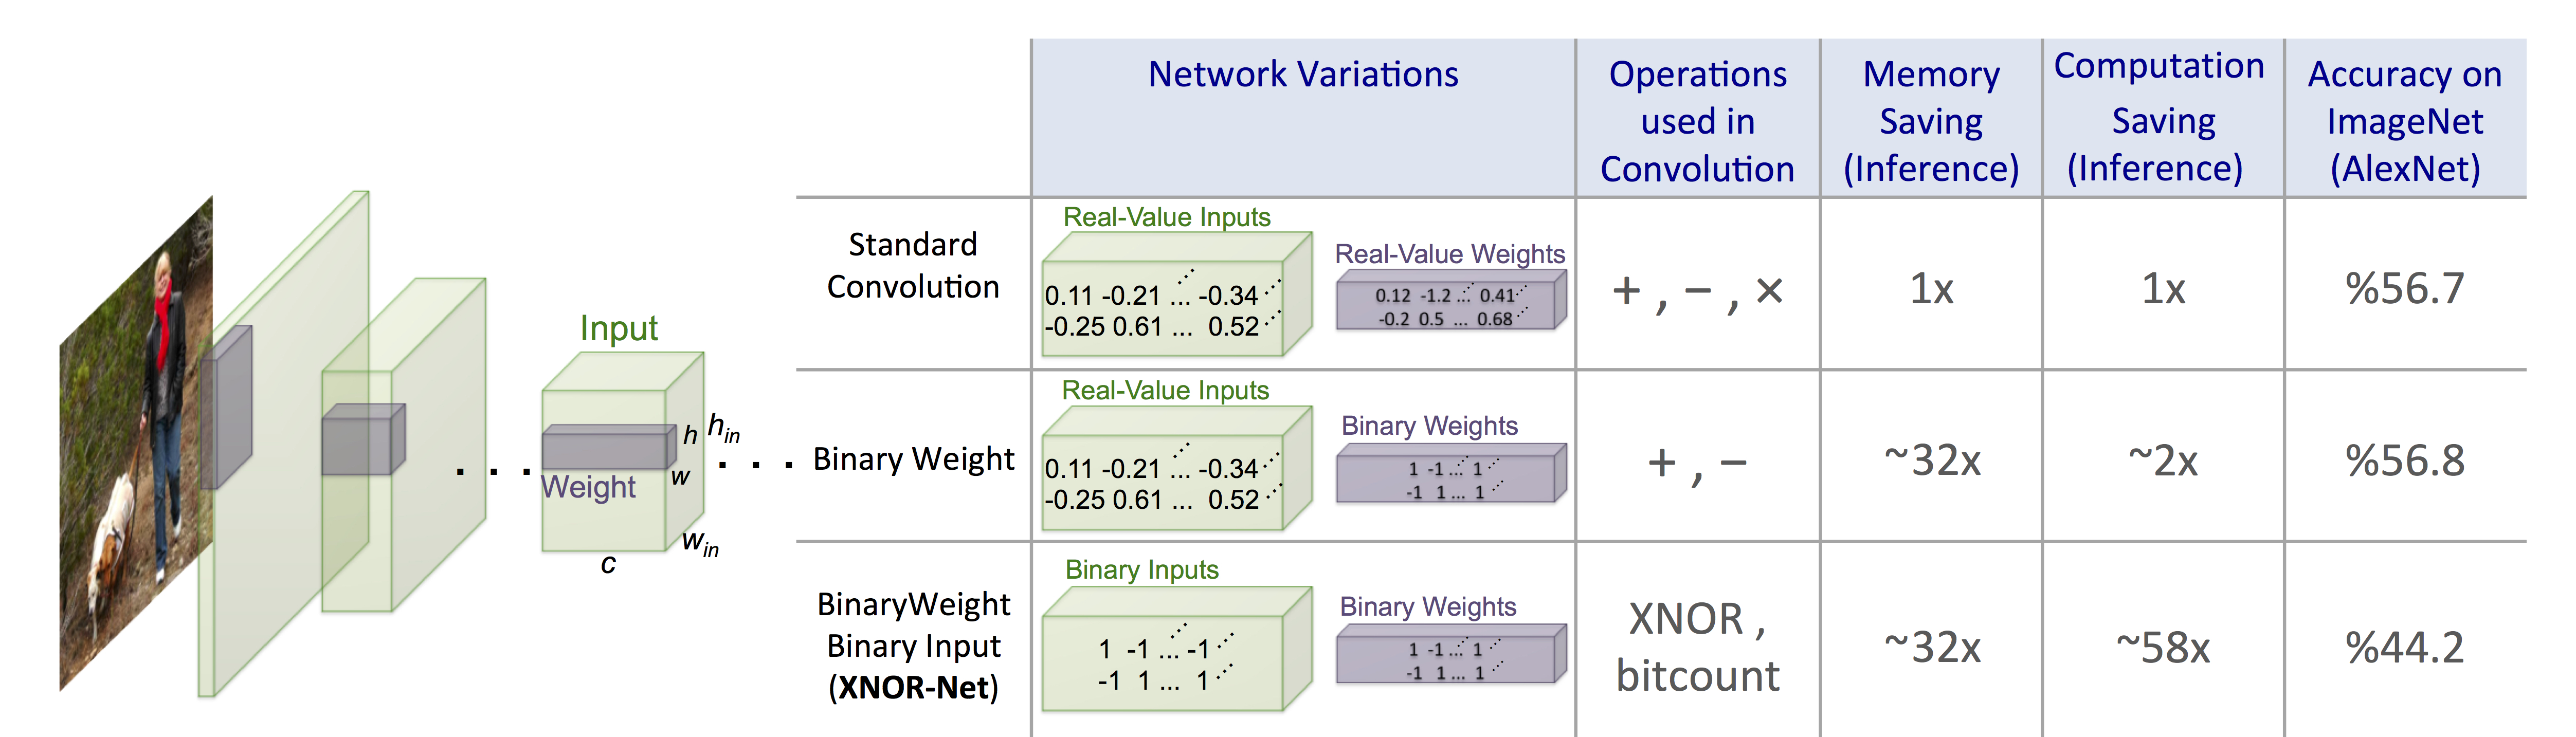
\includegraphics[width=1.0\textwidth]{binaryCNN}
	\caption[XOR-Net]
	{Two efficient variations of convolutional neural networks.
  Binary-Weight-Networks, when the weight filters contains binary values.
  XNOR-Networks, when both weigh and input have binary values. These
  networks are very efficient in terms of memory and computation, while
  being very accurate in natural image classification. This offers the
  possibility of using accurate vision techniques in portable devices
  with limited resources \citep{Rastegari2016}.}
  \label{fig:binaryCNN}
\end{figure}

The binary networks models proposed are simple, accurate, efficient, and
work on challenging visual tasks. In terms of precision, the classification
accuracy with a Binary-Weight-Network version of AlexNet is the same as the
full-precision AlexNet.

{\color{JungleGreen}
Añadir otros papers sobre arquitecturas para dispositivos portables:
\begin{itemize}
  \item MobileNets
  \item ShuffleNet
  \item NASNet
  \item PeleeNet
  \item Quantized CNNs for Mobile Devices {\color{blue}(Brief)} {\color{black}\citep{Wu2016}}
  \item Compression of deep CNNs {\color{blue}(Brief)} {\color{black}\citep{Kim2015}}
\end{itemize}
}

{\color{red}
Para la propuesta, considerar arquitecturas portables + arquitecturas
p/rostro + módulos funcionales.
}
